\section{Introduction}
Reinforcement Learning (RL) has shown great success in a wide range of applications including board games \cite{alphago}, strategy games \cite{alphastarblog}, energy systems \cite{chi_buildsys19}, robotics \cite{rl_robots_nn}, recommendation systems \cite{recommendation_rl}, hyperparameter selection \cite{effective_online_hyperparameter} etc. Typically, RL algorithms train by iteratively collecting the data by interacting with a simulator of the environment, and learning a model using the collected data. However, it takes a considerable amount of time to train a reinforcement learning agent to converge. This is because: 1) the speed of data collection is limited by the complexity of the environment simulator which needs to accurately represent the real world physical system; 2) the large state space needed to represent a typical real-world physical system makes it necessary to gather a large amount of data to successfully train a RL agent.  We show the training time versus the size of the state space of three popular environments used in RL training in Figure~\ref{fig:time_vs_state_space}. On Mujoco~\cite{mujoco}, which is a physics engine to simulate robotics, biomechanics, etc., it takes around 3 hours to train an agent using Pytorch \cite{pytorch} on a 4-core machine with a GTX 1060 GPU. On Atari~\cite{openai_gym}, which is a game simulator, it takes around 12 hours to train on the same machine. The state-of-the-art RL algorithm for playing Go --- AlphaGo Zero~\cite{alphago_zero} was trained on 4 TPUs \cite{tpu} for 21 days. Thus, developing faster reinforcement learning algorithms is an important research direction.


%1) the speed of data collection by interacting with the environment is constrained by hardware and rules (e.g. self-driving cars can drive at most 65 MPH in freeway at Los Angeles.); 2) the large state space makes it necessary to gather large amount of data to successfully train a reinforcement learning agent. 


 
%It takes around 3 hours to train an agent to tackle Mujoco \cite{mujoco} tasks using Pytorch \cite{pytorch} on a 4-core machine with a GTX 1060 GPU. 
%It takes around 12 hours to tackle Atari games \cite{openai_gym} on the same machine. 
%The state-of-the-art AlphaGo Zero \cite{alphago_zero} was trained on 4 TPUs \cite{tpu} for 21 days. Due to the computational expensiveness, developing parallel algorithms to accelerate the reinforcement learning algorithms becomes promising and critical.

Prior work tackles this problem by deploying parallel actors that can collect data simultaneously \cite{gorila, apex, a3c, impala}. \cite{gorila} introduces a parallel framework for Deep Q Network (DQN) \cite{dqn}. 
It accelerates the training by using independent actors collecting data asynchronously. The data is stored in a shared replay buffer. 
Meanwhile, parallel learners sample data uniformly from the replay buffer and compute the gradients. 
The gradients are sent to the central parameter server \cite{parameter_server} for neural network weights update.
\cite{apex} improves the performance of \cite{gorila} by using Prioritized Replay Buffer so that important data is sampled with higher weights to accelerate the training.

In these works, Replay Buffer management becomes a limiting factor in achieving high scalability when increasing parallelism. Improving the performance of parallel Replay Buffer management via techniques such as careful data structure design or low overhead thread-level synchronization has not received much attention. In this work, we optimize the implementation of Replay Buffer management and propose a framework for generating scalable reinforcement learning implementations. The generated RL implementations are composed of parallel actors and learners executing on computing platforms such as CPUs, GPUs, or FPGAs with Replay Buffer management executing on a CPU platform. We illustrate our framework by generating RL algorithms targeting a multi-core platform. Our key contributions are summarized as follows:
\begin{itemize}
    \item We propose a new data structure for the Prioritized Replay Buffer based on $K$-ary sum tree that supports asynchronous parallel insertions, sampling and priority update.
    \item We propose a novel data layout to store the nodes of the sum tree to minimize the number of cache misses.
    \item We propose \textit{lazy writing} mechanism to minimize the thread-level synchronization overhead of various operations of the Replay Buffer.
    \item Given a hardware configuration, our framework automatically decides the number of actors and learners such that the desired ratio between the throughput of the data collection and the throughput of the learning is achieved.
    \item Our framework supports a wide range of reinforcement learning algorithms including DQN \cite{dqn}, DDQN \cite{double_q_learning}, DDPG \cite{ddpg}, TD3 \cite{td3}, SAC \cite{sac}, etc.
  %  \item Given hardware resources, we perform design space exploration to determine the number of cores to run actors and the number of cores to run learners such that the throughput of the data collection matches the throughput of the learning.
    \item We demonstrate the effectiveness of our framework in accelerating RL algorithms by performing experiments on CPU + GPU platforms using OpenAI \cite{openai_gym} benchmarks. Our results show that the performance of our $K$-ary sum tree based Prioritized Replay Buffer improves the baseline implementations by around 4x$\sim$100x. Our proposed synchronization optimizations improve the performance by around 2x$\sim$4.4x compared with using a global lock. By plugging our Replay Buffer implementation into existing open source reinforcement learning frameworks, we achieve 1.19x$\sim$1.75x speedup for various algorithms.
\end{itemize}



%This is because these works lack detailed 


%Most prior works are either specialized for a particular algorithm or lack detailed synchronization mechanisms and data structure designs that support parallelism.
%In this work, we propose a framework for generating scalable reinforcement learning implementations on multicore platforms.
%Our key contributions are summarized as follows:


\begin{figure}
    \centering
    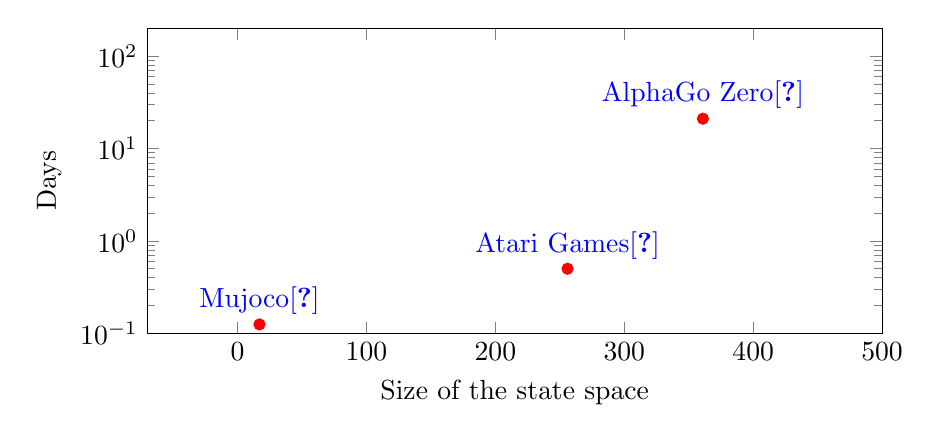
\begin{tikzpicture}
        \begin{axis}[
            ymode=log,
            xmin = -70, xmax = 500,
            ymin = 0.1, ymax = 200,
            xlabel={Size of the state space},
            ylabel={Days},
            % grid = both,
            % xmajorgrids=true,
            % major grid style = {lightgray},
            % minor grid style = {lightgray},
            width = 0.9\linewidth,
            height = 0.45\linewidth,
            nodes near coords=\pgfplotspointmeta,
            point meta=explicit symbolic
        ]
        \addplot[scatter,only marks,mark options={scale=1,fill=red,draw=red},color=blue] table [meta index=2] {
        4 0.01 CartPole
        17 0.125 Mujoco\cite{openai_gym}
        256 0.5 Atari\ Games\cite{openai_gym}
        361 21 AlphaGo\ Zero\cite{alphago_zero}
        };  
        \end{axis}
    \end{tikzpicture}
    \caption{Training time of various environments versus the size of the state space}
    \label{fig:time_vs_state_space}
\end{figure}
